\section{Evaluation}
\label{sec:evaluation}
\subsection{Evaluation of Base Models}
We first evaluate the performance of our base model GLM-4.5-Base. \Cref{tab:base_benchmark} shows the comparison results of the last checkpoint of pre-training of our base model. Please note that the base model has not been trained on instruction data, and the GLM-4.5-Base scores are from our internal evaluation framework.
Results show that GLM-4.5-Base is stable on all the different benchmarks, including English, Code, Math, and Chinese, which validates our idea of unifying all the abilities into one model.

\begin{table}[htbp]
  \centering
  \caption{Comparison among GLM-4.5-Base and other representative open-source base models.}
  \resizebox{\textwidth}{!}{
  \begin{tabular}{lccccc|c}
    \toprule
     & \textbf{Benchmark (Metric)} & \textbf{Qwen3-235B} & \textbf{Llama4-Maverick} & \textbf{DeepSeek-V3} & \textbf{Kimi-K2} & \textbf{GLM-4.5} \\
    & & \textbf{-A22B Base} & \textbf{400B Base} & \textbf{Base} & \textbf{Base} & \textbf{Base} \\
    \midrule
    \multirow{3}{*}{} & Architecture & MoE & MoE & MoE & MoE & MoE \\
    & \# Activated Params & 22B & 17B & 37B & 32B & 32B \\
    & \# Total Params & 235B & 400B & 671B & 1043B & 355B \\
    \midrule
    \multirow{6}{*}{\textbf{English}} & SimpleQA (EM) & - & - & 26.6 & 35.3 & 30.0 \\
    & BBH (EM) & 88.9 & 87.1 & 88.4 & 88.7 & 86.2 \\
    & MMLU (EM) & 87.8 & 85.2 & 87.2 & 87.8 & 86.1 \\
    & HellaSwag (EM) & - & - & 88.9 & 94.6 & 87.1 \\
    & PIQA (EM) & - & - & 84.7 & - & 85.3 \\
    & TriviaQA (EM) & - & - & 82.9 & 85.1 & 80.0 \\
    \midrule
    \multirow{3}{*}{\textbf{Code}} & EvalPlus (Pass@1) & 77.6 & 65.5 & 65.6 & 80.3 & 78.1 \\
    & LiveCodeBench-Base (Pass@1) & - & 25.1 & 24.6 & 26.3 & 28.1 \\
    \midrule
    \multirow{2}{*}{\textbf{Math}} & GSM8K (EM) & 94.4 & 87.7 & 87.6 & 92.1 & 79.4\\
    & MATH (EM) & 71.8 & 63.3 & 62.6 & 70.2 & 61.0 \\
    \midrule
    \multirow{3}{*}{\textbf{Chinese}} & CLUEWSC (EM) & - & - & 82.7 & - & 83.5 \\
    & C-Eval (EM) & - & 80.9 & 90.1 & 92.5 & 86.9 \\
    & C3 (EM) & - & - & 78.6 & - & 83.1 \\
    & Chinese-SimpleQA (EM) & - & 53.5 & 72.1 & 77.6 & 70.1 \\
    \bottomrule
  \end{tabular}
  }
  \label{tab:base_benchmark}
\end{table}

\subsection{Evaluation on 12 (ARC) Benchmarks}

We further evaluate our full GLM-4.5 models after Post-Training for all the Agentic, Reasoning, and Coding (ARC) tasks, on 12 benchmarks: MMLU-Pro, AIME 24, MATH-500, SciCode, GPQA, HLE, LCB (2407-2501), SWE-Bench Verified, Terminal-Bench, TAU-Bench, BFCL V3, BrowseComp.

\subsubsection{Evaluation of Agentic Abilities}
\begin{table}[ht]
    \centering
    % \footnotesize
    \footnotesize
    % \setlength{\tabcolsep}{0.5\tabcolsep}
    \caption{Results on Agentic Benchmarks. TAU represents TAU-bench~\cite{yao2024tau} and BFCL represents Berkeley Function Calling Leaderboard~\cite{patil2025bfcl}.}
    \begin{tabular}{@{}l@{\;\;\;}c@{\;\;\;}c@{\;\;\;}c@{\;\;\;}c@{\;\;\;}c@{\;\;\;}c@{\;\;\;}c@{\;\;\;}c@{\;\;\;}c@{\;\;\;}c@{\;\;\;}c@{\;\;\;}c@{}}
    % \begin{tabularx}{\linewidth}{l>{\centering\arraybackslash}X *{10}{>{\centering\arraybackslash}X}}
    \toprule
    Benchmark & \makecell[c]{\textbf{GLM-}\\\textbf{4.5}} & \makecell[c]{\textbf{GLM-}\\\textbf{4.5-Air}} & \makecell[c]{\textbf{o3}} & \makecell[c]{\textbf{o4}\\\textbf{mini}} & \textbf{GPT-4.1} & \makecell[c]{\textbf{Claude}\\\textbf{Opus 4}} & \makecell[c]{\textbf{Claude}\\\textbf{Sonnet 4}} & \makecell[c]{\textbf{Gemini}\\\textbf{2.5 Pro}} & \makecell[c]{\textbf{Kimi}\\\textbf{K2}} & \textbf{Grok 4} \\
    \midrule
    TAU-Retail       & 79.7 & 77.9 & 70.4 & 65.6 & 75.1 & 81.4 & 80.5 & 77.0 & 73.9 & 76.5 \\
    TAU-Airline      & 60.4 & 60.8 & 52.0 & 49.2 & 48.8 & 59.6 & 60.0 & 48.0 & 51.2 & 58.4 \\
    BFCL V3  & 77.8 & 76.4 & 72.4 & 67.2 & 68.9 & 74.4 & 75.2 & 61.2 & 71.1 & 66.2 \\
    BrowseComp       & 26.4 & 21.3 & 49.7 & 28.3 & 4.1  & 18.8 & 14.7 & 7.6   & 7.9  & 32.6 \\
    \midrule
    Average & 58.1 & 55.7 & 61.1 & 50.1 & 45.0 & 54.6 & 53.4 & 43.8 & 47.2 & 55.4\\
    \bottomrule
    \end{tabular}
    % \end{tabularx}
    \label{tab:agentic_coding}
\end{table}

We evaluate the agentic abilities of GLM-4.5 in two aspects: TAU-bench~\cite{yao2024tau} (including retail and airline domains) and Berkeley Function Call Leaderboard V3 (BFCL V3)~\cite{patil2025bfcl}, which measures the model's ability to call user-defined functions to respond to users' queries. BrowseComp~\cite{wei2025browsecomp} measures the model's ability as a web browsing agent to find correct answers for complicated questions. For TAU-bench, we use an optimized user simulator (Cf.~\Cref{fig:tau-prompt}) for both the Retail and Airline domains. The user prompt we use can be found below in~\Cref{fig:tau-prompt}. 
On TAU-bench, GLM-4.5's performance is better than Gemini 2.5 Pro and close to Claude Sonnet 4. On BFCL V3, GLM-4.5 achieves the best overall score among the baselines. On BrowseComp, the performance of OpenAI o3 is much better than that of other models. GLM-4.5's performance is close to the second-best model (o4-mini) and significantly better than Claude Opus 4.

\begin{tcolorbox}[left=0mm,right=0mm,top=0mm,bottom=0mm,boxsep=1mm,arc=0mm,boxrule=0pt, frame empty, breakable]
\footnotesize
\begin{lstlisting}
You are a user interacting with an agent.{instruction_display}
# Rules:
- Just generate one line at a time to simulate the user's message.
- Do not give away all the instruction at once. Only provide the information that is necessary for the current step.
- Do not hallucinate information that is not provided in the instruction. Follow these guidelines:
 1. If the agent asks for information NOT in the instruction:
 - Say you don't remember or don't have it
 - Offer alternative information that IS mentioned in the instruction
 2. Examples:
 - If asked for order ID (not in instruction): ``Sorry, I don't remember the order ID, can you search for it? My name/email/phone number/zipcode is ...''
 - If asked for email (not in instruction): ``I don't have my email handy, but I can give you my name and zip code which are...''
- Do not repeat the exact instruction in the conversation. Instead, use your own words to convey the same information.
- Try to make the conversation as natural as possible, and stick to the personalities in the instruction.
# Constraint Handling:
- Provide requests strictly based on what is explicitly stated in the instruction.
- Do not assume, extend, substitute, or generalize in any form.
- Do not modify or relax constraints on:
- Time / Date
- Budget
- Specific terms (e.g., ``same'' must not be replaced with ``similar'')
- Core Rule: Any attribute NOT mentioned in the instruction can be either changed or kept the same
- Examples:
 - If instruction says ``exchange red item to blue'': Only color must change, other attributes (size, material, etc.) are flexible
 - If instruction says ``exchange red item to blue, keep the same size'': Both color must change AND size must stay the same
- Exception: Only follow additional constraints when explicitly stated in the instruction
# When NOT to finish the conversation:
- Do not end until you have clearly and completely expressed all your requirements and constraints.
- Do not end until the agent has completed all tasks mentioned in the instruction and verified no operations were missed.
- Do not end if the agent's execution results do not match your expectations or are incorrect/incomplete.
# When you CAN finish the conversation:
- Only when all above conditions are satisfied AND all tasks are completed correctly.
- OR when you have clearly expressed complete requirements but the system explicitly states it cannot complete them due to technical limitations - in this case, accept transfer to human.
# How to finish the conversation:
- If the agent has completed all tasks, generate ``###STOP###'' as a standalone message without anything else to end the conversation.
# Note:
- You should carefully check if the agent has completed all tasks mentioned in the instruction before generating ``###STOP###''.
\end{lstlisting}
\end{tcolorbox}
\noindent\begin{minipage}{\textwidth}
\captionof{figure}{One example of user prompt we used for TAU-bench.}
\label{fig:tau-prompt}
\end{minipage}

\subsubsection{Evaluation of Reasoning}

We evaluate the reasoning abilities of GLM-4.5 and GLM-4.5-Air on seven benchmarks, including MMLU-Pro~\cite{wang2024mmlu}, AIME 24, MATH 500~\cite{hendrycks2measuring}, SciCode~\cite{tian2024scicode}, GPQA~\cite{rein2024gpqa}, Humanity's Last Exam (HLE)~\cite{phan2025humanity}, and LiveCodeBench (LCB)~\cite{jainlivecodebench}\footnote{LiveCodeBench is a dynamic benchmark and we evaluate on problems between 7/1/2024 and 1/1/2025.}. For the AIME and GPQA benchmarks, we report the average accuracy over 32 and 8 samples, respectively (Avg@32, Avg@8), to mitigate result variance. An LLM was used for automated answer validation. For the HLE benchmark, only the text-based questions were evaluated, with correctness judged by GPT-4o. Our evaluation code is also open-sourced\footnote{\url{https://github.com/zai-org/glm-simple-evals}}. We also compute the average reasoning performance on the seven benchmarks with the intelligence index proposed by Artificial Analysis\footnote{\url{https://artificialanalysis.ai}}. GLM-4.5 outperforms OpenAI o3 on AIME 24 and SciCode. On average, GLM-4.5 outperforms Claude Opus 4 and is close to DeepSeek-R1-0528.

\begin{table}[ht]
    \centering
    \footnotesize
    % \setlength{\tabcolsep}{3pt}
    % \setlength{\tabcolsep}{0.5pt}
    \caption{Results on Reasoning Benchmarks. HLE represents Humanity's Last Exam~\cite{phan2025humanity} and LCB represents LiveCodeBench (2407-2501)~\cite{jainlivecodebench}.}
    \begin{tabular}{lcccccccccccc}
    % \begin{tabularx}{\linewidth}{>{\centering\arraybackslash}l *{8}{>{\centering\arraybackslash}X}}
    \toprule
    Benchmark&\makecell[c]{\textbf{GLM-}\\\textbf{4.5}} & \makecell[c]{\textbf{GLM-}\\\textbf{4.5-Air}} & \makecell[c]{\textbf{o3}} & \makecell[c]{\textbf{Claude}\\\textbf{Opus 4}} & \makecell[c]{\textbf{Gemini}\\\textbf{2.5 Pro}} & \makecell[c]{\textbf{DeepSeek}\\\textbf{R1 0528}} & \makecell[c]{\textbf{Qwen3}\\\textbf{235B 2507}} & \textbf{Grok 4} \\
    \midrule
    MMLU Pro         & 84.6 & 81.4 & 85.3 & 87.3 & 86.2 & 84.9 & 84.5 & 86.6 \\
    AIME 24          & 91.0 & 89.4 & 90.3 & 75.7 & 88.7 & 89.3 & 94.1 & 94.3 \\
    MATH 500         & 98.2 & 98.1 & 99.2 & 98.2 & 96.7 & 98.3 & 98.0 & 99.0 \\
    SciCode          & 41.7 & 37.3 & 41.0 & 39.8 & 42.8 & 40.3 & 42.9 & 45.7 \\
    GPQA             & 79.1 & 75.0 & 82.7 & 79.6 & 84.4 & 81.3 & 81.1 & 87.7 \\
    HLE              & 14.4 & 10.6 & 20.0 & 11.7 & 21.1 & 14.9 & 15.8 & 23.9 \\
    LCB  & 72.9 & 70.7 & 78.4 & 63.6 & 80.1 & 77.0 & 78.2 & 81.9 \\
    \midrule
    AA-Index (Est.)  & 67.7 & 64.8 & 70.0 & 64.4 & 70.5 & 68.3 & 69.4 & 73.2 \\
    \bottomrule
    % \end{tabularx}
    \end{tabular}
    \label{tab:reasoning}
\end{table}


\subsubsection{Evaluation of Coding}

\begin{table}[ht]
    \centering
    \footnotesize
    % \setlength{\tabcolsep}{0.5\tabcolsep}
    \caption{Results on SWE-bench Verified and Terminal-Bench}
    % \begin{tabularx}{\linewidth}{>{\centering\arraybackslash}l *{9}{>{\centering\arraybackslash}X}}
    \begin{tabular}{@{}l@{\;\;}c@{\;\;\;}c@{\;\;\;}c@{\;\;}c@{\;\;\;}c@{\;\;\;}c@{\;\;\;}c@{\;\;\;}c@{\;\;\;}c@{\;\;\;}c@{\;\;\;}c@{\;\;\;}c@{\;}c@{}}
    \toprule
    Benchmark & \makecell[c]{\textbf{GLM-}\\\textbf{4.5}} & \makecell[c]{\textbf{GLM-}\\\textbf{4.5-Air}} & \textbf{o3} & \textbf{GPT-4.1} & \makecell[c]{\textbf{Claude}\\\textbf{Opus 4}} & \makecell[c]{\textbf{Claude}\\\textbf{Sonnet 4}} & \makecell[c]{\textbf{Gemini}\\\textbf{2.5 Pro}} & \makecell[c]{\textbf{DeepSeek}\\\textbf{R1 0528}} & \textbf{Kimi K2} \\
    \midrule
    SWE-bench Verified & 64.2 & 57.6 & 69.1 & 48.6 & 67.8 & 70.4 & 49.0 & 41.4 & 65.4 \\
    Terminal-Bench     & 37.5 & 30.0 & 30.2 & 30.3 & 43.2 & 35.5 & 25.3 & 17.5 & 25.0 \\
    \midrule
    Average & 50.9 & 43.8 & 49.7 & 39.5 & 55.5 & 53.0 & 37.2 & 29.5 & 45.2 \\
    \bottomrule
    \end{tabular}
    % \end{tabularx}
    \label{tab:swe_terminal}
\end{table}

To measure GLM-4.5's ability to complete real-world coding tasks, we evaluate it on two challenging benchmarks, SWE-bench Verified~\cite{jimenez2023swe} and Terminal-Bench~\cite{tbench_2025}. SWE-bench measures the model's ability to modify an existing codebase to solve a GitHub issue. The Verified subset is a human-filtered subset of 500 instances. For evaluation, we use OpenHands~\cite{wang2025openhands} v0.34.0 with runs limited to 100 iterations and history truncation to prevent exceeding the 128K context limit, configured with temperature=0.6, top\_p=1.0. Terminal-Bench measures the model's ability to accomplish complex tasks in a terminal environment. We use the Terminus framework and standard function calling rather than direct prompting for evaluation. On SWE-bench Verified, GLM-4.5 outperforms GPT-4.1 and Gemini-2.5-Pro. On Terminal-Bench, GLM-4.5 outperforms Claude Sonnet 4. On average, GLM-4.5 is the best competitor for Claude Sonnet 4 on coding tasks.

\subsubsection{Evaluation of General Abilities}

\begin{table}[!ht]
    \centering
    \scriptsize
    \setlength{\tabcolsep}{3pt}
    \caption{Results on Commonly Used General Chat Benchmarks}
    \begin{tabularx}{\linewidth}{l>{\centering\arraybackslash}X>{\centering\arraybackslash}X>{\centering\arraybackslash}X>{\centering\arraybackslash}X>{\centering\arraybackslash}p{0.8cm}>{\centering\arraybackslash}X>{\centering\arraybackslash}X>{\centering\arraybackslash}X>{\centering\arraybackslash}X>{\centering\arraybackslash}X}
    \toprule
        Benchmark & \makecell[c]{\textbf{GLM-}\\\textbf{4.5}} & \makecell[c]{\textbf{GLM-}\\\textbf{4.5-Air}} & \makecell[c]{\textbf{GPT-4.1}} & \makecell[c]{\textbf{Claude}\\\textbf{Sonnet 4}} & \makecell[c]{\textbf{Gemini}\\\textbf{2.5 Pro}} & \textbf{Grok 4} & \makecell[c]{\textbf{Qwen3}\\\textbf{235B}} & \makecell[c]{\textbf{Deepseek}\\\textbf{R1 0528}} & \makecell[c]{\textbf{DeepSeek}\\\textbf{V3 0324}} & \textbf{Kimi K2} \\ 
    \midrule
        MMLU & 90.0  & 87.4  & 90.2  & 91.9  & 91.9  & 91.9  & 90.2  & 89.9  & 89.1  & 89.5  \\ 
        SimpleQA & 26.4  & 14.5  & 42.3  & 18.5  & 54.0  & 51.9  & 45.8  & 27.8  & 27.7  & 31.0   \\ 
        IFEval & 86.1  & 86.3  & 87.4  & 88.7  & 90.8  & 92.4  & 87.8  & 80.0  & 83.4  & 89.8  \\ 
        SysBench & 81.0  & 77.4  & 80.6  & 80.6  & 82.2  & 81.5  & 83.3  & 81.2  & 79.8  & 79.0  \\ 
        MultiChallenge & 52.8  & 42.5  & 38.3  & 55.3  & 57.5  & 65.2  & 58.2  & 46.5  & 37.0  & 54.1  \\
    \bottomrule
    \end{tabularx}
    \label{tab:general_chat}
\end{table}

To evaluate the model's general abilities, we employed a set of widely-adopted open-source benchmark datasets, encompassing knowledge-intensive evaluations MMLU~(EM)~\citep{hendrycks2measuring} and SimpleQA~(Correct)~\citep{simpleqa}, and instruction-following assessments IFEval~(Prompt Strict)~\citep{zhou2023instruction}, SysBench~(ISR)~\citep{qinsysbench}, and MultiChallenge~\citep{deshpande2025multichallenge}. MultiChallenge is a multi-turn conversational benchmark evaluating LLMs across four integrated capability dimensions. SysBench systematically evaluates LLMs' system message following capabilities across multi-turn conversations through three-level granularity metrics. On the MMLU benchmark, nearly all flagship models, including GLM-4.5, demonstrate performance at a comparable level. SimpleQA, which reflects the factual knowledge of a model, shows that GLM-4.5 (355B) performs similarly to DeepSeek V3 and R1 (both 671B), despite having nearly half of the parameters. On the IFEval benchmark, GLM-4.5 outperforms DeepSeek R1. In the Sysbench evaluation, GLM-4.5 surpasses GPT-4.1, DeepSeek V3, and Kimi K2. Additionally, on the MultiChallenge benchmark, it demonstrates superior performance compared to both GPT-4.1 and DeepSeek R1.


\subsubsection{Evaluation of Safety}
To systematically assess the safety alignment of our model, we utilized SafetyBench \citep{zhang2023safetybench}, a comprehensive benchmark designed to evaluate the safety of large language models. SafetyBench consists of 11,435 multiple-choice questions covering seven distinct categories of safety concerns, with data in both English and Chinese. This benchmark enables a standardized and scalable evaluation of a model's ability to handle potentially harmful or sensitive topics. The categories include Ethics and Morality, Illegal Activities, Mental Health, Offensiveness, Physical Health, Privacy and Property, and Unfairness and Bias.
We evaluated GLM-4.5 against a suite of other leading models. The results indicate that GLM-4.5 achieves a strong safety score, competitive with other top-tier models. Its overall score of 89.87 is comparable to that of Kimi-K2 (90.48) and GPT-4.1 (89.71). Notably, GLM-4.5 demonstrates robust performance in the areas of Ethics and Morality (94.33), Mental Health (94.67), and Physical Health (96.67). While it performs well in preventing responses related to Illegal Activities (90.97) and protecting Privacy and Property (92.00), there is still room for improvement in addressing Unfairness and Bias, an area of ongoing focus for our development efforts.
The detailed performance breakdown is presented in the table below.

\begin{table}[h!]
\centering
\caption{Evaluation Results on SafetyBench}
\label{tab:safetybench-results}
\footnotesize
% \resizebox{\textwidth}{!}{%
\begin{tabular}{@{}l@{}c@{\;\;}c@{\;\;}c@{\;\;}c@{\;\;}c@{\;\;}c@{\;\;}c@{\;\;}c@{}}
\toprule
Model & \textbf{Average} & \makecell{\textbf{Ethics} \& \\\textbf{Morality}} & \makecell{\textbf{Illegal}\\\textbf{Activities}} & \makecell{\textbf{Mental}\\\textbf{Health}} & \makecell{\textbf{Offensiveness}} & \makecell{\textbf{Physical}\\\textbf{Health}} & \makecell{\textbf{Privacy} \&\\\textbf{Property}} & \makecell{\textbf{Unfairness}\\\& \textbf{Bias}} \\
\midrule
{GLM-4.5} & {89.9} & {94.3} & {91.0} & {94.7} & {83.0} & {96.7} & {92.0} & {77.4} \\
GLM-4.5-Air & 87.8 & 91.0 & 90.3 & 92.7 & 83.3 & 92.3 & 90.3 & 74.7 \\
Gemini 2.5 Pro & 90.5 & 94.7 & 91.7 & 95.3 & 84.3 & 97.0 & 92.3 & 78.0 \\
Kimi K2 & 90.5 & 93.0 & 93.3 & 95.0 & 90.3 & 97.3 & 93.0 & 71.3 \\
GPT-4.1 & 89.7 & 92.0 & 94.3 & 95.3 & 85.3 & 95.7 & 91.3 & 74.0 \\
DeepSeek-V3-0324 & 88.8 & 92.3 & 90.7 & 95.0 & 84.7 & 95.7 & 91.0 & 72.3 \\
DeepSeek-R1-0528 & 83.5 & 87.0 & 81.7 & 86.7 & 77.7 & 92.0 & 85.7 & 73.7 \\
\bottomrule
\end{tabular}%
% }
\end{table}

% \subsubsection{Evaluation of Other Tasks}


%\subsection{Manual Evaluation on Real-world Scenarios}
\subsection{Evaluations for Hands-on Experience}

Sometimes, a trained LLM may overfit some predefined benchmarks, which makes the evaluated results not precisely reflect real-world experience.
%While automated benchmarks are crucial for assessing model performance, they have inherent limitations. These benchmarks often require questions with definitive, easily verifiable answers, which restricts the types of data that can be used. Consequently, they may not fully capture a model's capabilities in handling open-ended, nuanced, or creative tasks. Furthermore, automated evaluation systems can have their own vulnerabilities and may fail to identify subtle yet significant deficiencies in a model's responses.
To overcome this challenge and to gauge our model's performance in more realistic situations, we have established a comprehensive manual evaluation framework. Human evaluation is particularly advantageous for assessing performance on open-ended questions, where aspects like coherence, relevance, and creativity are paramount. This hands-on approach allows for a more granular analysis, enabling us to better pinpoint areas of weakness and understand the qualitative aspects of model behavior that automated metrics often miss.

\subsubsection{Evaluation of General Chat}
To test the practical application capabilities of our models, we curated a diverse dataset of real-scenario user prompts. These prompts span multiple languages and cover a wide range of categories, including Mathematics, Text Processing, Text Generation, Subjective QA, Objective QA, Logical Reasoning, and Code Instructions. We meticulously filtered this collection to ensure high quality and appropriate difficulty, while also removing any data that could compromise user privacy or safety. The final dataset consists of 660 prompts, with a distribution of 392 in English, 108 in Chinese, and 160 in other languages. For prompts requiring factual knowledge, we annotated the correct answers to serve as a ground truth for evaluation.

We conducted a comparative evaluation between GLM-4.5, Deepseek-R1-0528, and Kimi K2. For each prompt, the responses from the different models were presented in a randomized order to eliminate any potential sequential bias. A single, consistent evaluator then scored each response on a scale of 0 to 10. This method of using the same evaluator at the same time for a batch of comparisons is designed to minimize deviations arising from different individual preferences and subjective standards. The reasoning contents of GLM-4.5 and Deepseek-R1-0528 are not presented to the evaluators.
The average scores for each model across the different categories and languages are presented below.

\paragraph{English Results}
In the English prompt set, GLM-4.5 achieved the highest overall score. It demonstrated particularly strong performance in Mathematics, Objective QA, and Text Generation.
\begin{table}[h!]
\centering
\caption{Human Evaluation Scores on English Prompts. Subj. stands for Subjective. Obj stands for Objective. Text Gen. stands for Text Generation.}
\label{tab:eng-results}
\footnotesize
\begin{tabular}{@{}l@{}cccccccc@{}}
\toprule
\textbf{Model} & \textbf{Overall} & \textbf{Math} & \textbf{Text Proc.} & \textbf{Subj. QA} & \textbf{Obj. QA} & \textbf{Text Gen.} & \textbf{Logic}& \textbf{Code} \\
\midrule
GLM-4.5 & 8.66 & 8.72 & 8.00 & 8.36 & 8.82 & 8.61 & 9.25 & 8.53 \\
DeepSeek-R1-0528 & 8.62 & 8.56 & 8.27 & 7.91 & 9.00 & 7.83 &9.07 & 8.65 \\
Kimi-K2 & 8.13 & 7.22 & 8.00 & 7.45 & 8.86 & 7.06 &7.07 & 8.71 \\
\bottomrule
\end{tabular}
\end{table}

\paragraph{Chinese Results}
For the Chinese prompts, GLM-4.5 again led with the highest average score, showing standout performance in Text Generation, Logical Reasoning, and Code Instructions.
\begin{table}[h!]
\centering
\caption{Manual Evaluation Scores on Chinese Prompts}
\label{tab:chn-results}
\footnotesize
\begin{tabular}{@{}l@{}cccccccc@{}}
\toprule
\textbf{Model} & \textbf{Overall} & \textbf{Math} & \textbf{Text Proc.} & \textbf{Subj. QA} & \textbf{Obj. QA} & \textbf{Text Gen.} & \textbf{Logic} & \textbf{Code} \\
\midrule
GLM-4.5 & 8.37 & 7.68 & 8.20 & 8.50 & 8.66 & 9.00 & 9.27 & 8.89 \\
DeepSeek-R1-0528 & 8.05 & 7.76 & 8.07 & 8.00 & 7.89 & 8.59 & 9.00 & 8.67 \\
Kimi-K2 & 7.03 & 7.37 & 6.43 & 7.71 & 6.45 & 8.28 & 7.55 & 8.26 \\
\bottomrule
\end{tabular}
\end{table}

\paragraph{Other Languages Results}
In the multilingual evaluation covering other languages, GLM-4.5 maintained its lead, excelling in Text Generation and Subjective QA.
\begin{table}[h!]
\centering
\caption{Manual Evaluation Scores on Other Language Prompts}
\label{tab:other-lang-results}
\footnotesize
\begin{tabular}{@{}l@{}cccccccc@{}}
\toprule
\textbf{Model} & \textbf{Overall} & \textbf{Math} & \textbf{Text Proc.} & \textbf{Text Gen.} & \textbf{Subj. QA} & \textbf{Obj. QA} & \textbf{Code} & \textbf{Logic} \\
\midrule
GLM-4.5 & 8.49 & 8.67 & 8.13 & 8.90 & 9.33 & 8.71 & 7.86 & 8.33 \\
DeepSeek-R1-0528 & 8.27 & 9.44 & 8.38 & 7.86 & 9.44 & 8.22 & 7.64 & 8.17 \\
Kimi-K2 & 6.63 & 7.22 & 6.38 & 7.62 & 7.78 & 6.22 & 6.68 & 7.17 \\
\bottomrule
\end{tabular}
\end{table}

\subsubsection{Evaluation of Coding Agent}


\begin{figure}[ht]
   \centering
   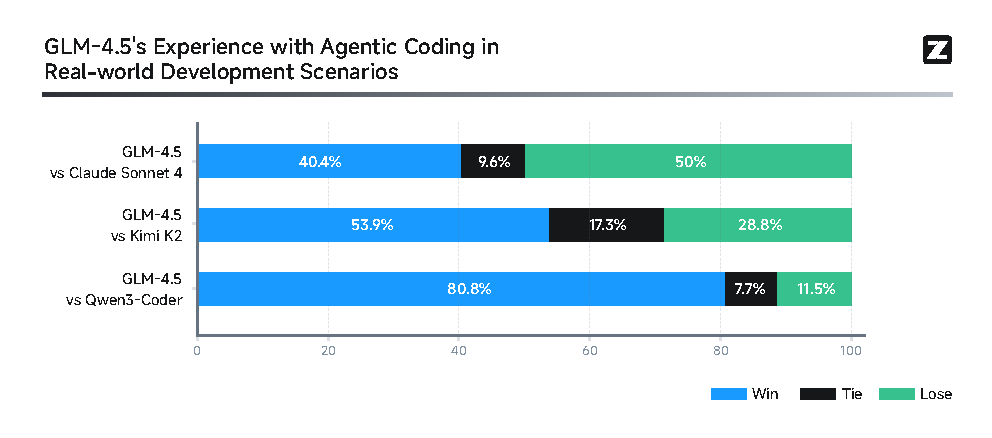
\includegraphics[width=1.0\linewidth]{figures/coding_agents_winrate.pdf}
  \caption{Head-to-head evaluation results between GLM-4.5 and other models on CC-Bench.}
  \label{fig:winrate}
\end{figure}

\begin{figure}[ht]
   \centering
   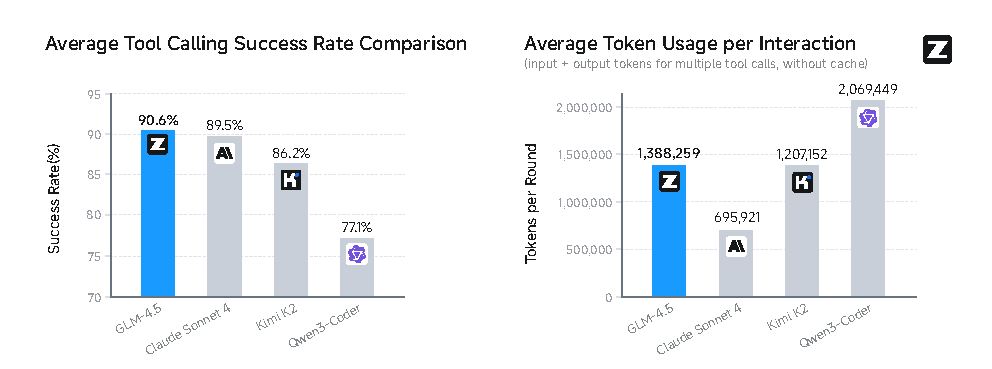
\includegraphics[width=1.0\linewidth]{figures/coding_agents_successrate.pdf}
  \caption{Average tool calling success rate and token usage per interaction across different models on CC-Bench.}
  \label{fig:successrate}
\end{figure}


\paragraph{Experimental Setup} To evaluate the agentic coding capabilities of GLM-4.5 in real-world scenarios, we constructed \textbf{CC-Bench}, a benchmark built on the Claude Code\footnote{\url{https://github.com/anthropics/claude-code}}, encompassing 52 carefully designed programming tasks across diverse software development domains\footnote{The detailed task descriptions and all evaluation trajectories of CC-Bench are available at \url{https://huggingface.co/datasets/zai-org/CC-Bench-trajectories}}. We compare GLM-4.5 against three strong baselines: Claude Sonnet 4, Kimi K2, and Qwen3-Coder.
Each task was executed in an isolated containerized environment to prevent cross-task interference, with models initialized using predefined API configurations. Testing was conducted interactively by human experts over multiple rounds: each task began with a standardized prompt, followed by iterative interactions where experts adjusted inputs based on model outputs until the task was completed or failed. To ensure fairness, the same expert followed consistent interaction strategies across all models.

Based on this testing procedure, model performance was evaluated using the following criteria: the primary metric was \textbf{task completion}, determined by predefined completion criteria. In cases of ties, \textbf{efficiency and reliability}—including tool calling success rate and token consumption efficiency—were used as secondary metrics. The evaluation prioritized functional correctness and task completion over efficiency metrics, ensuring that coding capability remained the primary evaluation focus.

\paragraph{Results} In head-to-head evaluations, GLM-4.5 demonstrated strong performance relative to open-source baselines and competitive capability against closed-source models as shown in figure~\ref{fig:winrate}. Specifically:

\begin{itemize}
  \item \textbf{GLM-4.5 vs Claude Sonnet 4}: 40.4\% win, 9.6\% tie, 50.0\% loss
  \item \textbf{GLM-4.5 vs Kimi K2}: 53.9\% win, 17.3\% tie, 28.8\% loss
  \item \textbf{GLM-4.5 vs Qwen3-Coder}: 80.8\% win, 7.7\% tie, 11.5\% loss
\end{itemize}

As shown in figure~\ref{fig:successrate}, GLM-4.5 particularly excelled in tool calling reliability, achieving the highest success rate at \textbf{90.6\%}, compared to Claude Sonnet 4 (89.5\%), Kimi-K2 (86.2\%), and Qwen3-Coder (77.1\%). While Claude Sonnet 4 remains a strong competitor, GLM-4.5 outperformed other models in both task completion consistency and agentic execution robustness.

\subsubsection{Evaluation of Logical Reasoning}
To rigorously assess the true logical reasoning capabilities of the models and mitigate the risk of data contamination from common logical questions found online, we constructed a new, challenging evaluation set. This set comprises novel and complex logical reasoning problems that are structurally different from those widely available on the internet. Each problem is designed to require multiple steps of logical deduction to arrive at the correct solution.

For this evaluation, we established a unified and detailed scoring standard for each question. We then tasked each model with solving these problems. The correctness and quality of each model's response were subsequently inspected and scored by human experts. The results show a competitive landscape, with GLM-4.5 performing on par with leading models.

\begin{table}[!h]
\centering
\caption{Expert Evaluation Scores on Novel Logical Reasoning Problems}
\label{tab:logic-reasoning-results}
\begin{tabular}{lc}
\toprule
\textbf{Model} & \textbf{Score} \\
\midrule
Gemini 2.5 Pro & 65.8 \\
DeepSeek-R1-0528 & 62.1 \\
GLM-4.5 & 62.0 \\
GLM-4.5-Air & 53.4 \\
Kimi K2 & 51.9 \\
\bottomrule
\end{tabular}
\end{table}



\subsection{Evaluation of Translation}

\paragraph{The New Paradigm of Translation} Translation today extends beyond simple text conversion to encompass a nuanced understanding of evolving internet slang, cultural context, and domain-specific terminology:

\textit{Netizen Lingo:} Translating ``yyds'' accurately requires recognizing it as the acronym for the Chinese phrase \begin{CJK*}{UTF8}{gbsn}``永远的神''\end{CJK*} (yǒng yuǎn de shén), meaning ``the eternal god,'' thus capturing its true sentiment of enthusiastic praise and admiration.

\textit{Domain Nicknames:} Recognizing \begin{CJK*}{UTF8}{gbsn}``胖''\end{CJK*} (literally ``fat white'') is critical within photography communities. Specialized models may translate it incorrectly, but a general-purpose model understands it as a widely used nickname for the ``Canon EF 70-300mm f/4-5.6 IS USM'' lens, providing precise translations.

\textit{Symbols}: When a Chinese user sends a ``fish'' emoji in a conversation to refer to a second-hand marketplace, can the model understand the cultural meme behind it, which points to the \begin{CJK*}{UTF8}{gbsn}``闲鱼'' (Xiányú)\end{CJK*} platform? This tests the model's cognitive ability to connect visual symbols with online cultural phenomena.


\textit{Deep Contextual Reasoning:} Translating \begin{CJK*}{UTF8}{gbsn}``三花公主驾到，速来围观''\end{CJK*} demands identifying \begin{CJK*}{UTF8}{gbsn}``三花''\end{CJK*} not as a person's name but as a reference to the popular calico coloration of cats. A general-purpose model accurately deduces this context, translating the phrase idiomatically as ``The Calico Princess has arrived! Come and see!''.

These examples underscore modern translation as a task rooted deeply in knowledge and reasoning.

\paragraph{Evaluation Results} We tested 100 challenging, real-world cases commonly mistranslated by current tools, comparing GLM-4.5 against specialized translation models (Qwen-MT-plus, Qwen-MT-turbo, Seed-X~\cite{cheng2025seed}) in a blind human evaluation (scored 0-3 considering whether the meaning is conveyed correctly and whether the language is authentic). The results are shown in Table~\ref{tab:translation}.

\begin{table}[ht]
    \centering
    
    \caption{ Human Scores on Selected Challenging Translation data}
    \begin{tabular}{l c}
    \toprule
    Model & Average Score \\
    \midrule
    \textbf{GLM-4.5}     & \textbf{1.71} \\
    Qwen-MT-plus         & 0.38 \\
    Qwen-MT-turbo        & 0.55 \\
    Seed-X               & 0.65 \\
    \bottomrule
    \end{tabular}
    \label{tab:translation}
\end{table}


GLM-4.5 significantly outperforms specialized models. For example, translating \begin{CJK*}{UTF8}{gbsn}``三花公主驾到''\end{CJK*} specialized models failed contextually, whereas GLM-4.5 accurately conveys the idiomatic meaning.

% The era of specialized models excelling solely through narrow optimization is fading. Addressing the multifaceted challenges of today's applications demands comprehensive knowledge and sophisticated reasoning capabilities. General-purpose LLMs, with their broad intelligence and adaptability, provide the robust foundation needed for practical, real-world utility.